\documentclass[10pt,a4paper]{report}
\usepackage[utf8]{inputenc}
\usepackage{amsmath}
\usepackage{amsfonts}
\usepackage{bm}
\usepackage{amssymb}
\usepackage{float}
\usepackage{graphicx}
\usepackage{caption}
\usepackage{subfig}
\usepackage[table,xcdraw]{xcolor}
\usepackage{hyperref}

\graphicspath{{images/}}

\DeclareMathOperator*{\argmax}{arg\,max}
\DeclareMathOperator*{\argmin}{arg\,min}

\newcommand{\cmp}[1]{\bm{\tilde{#1}}}
\setcounter{tocdepth}{3}
\setcounter{secnumdepth}{3}

\author{Nicolò Brandizzi}
\title{Machine Learning Summary}


\begin{document}
\maketitle
\tableofcontents
\newpage



\newcommand{\braces}[1]{\lbrace{#1}\rbrace}

\chapter{Summaries}
\section{Intro}

ML is producing knowledge from data, learning a function $f:X\rightarrow Y$ that takes some input $x \in X$ and outputs $y \in Y$.\\
Learning $f$ means finding some approximation $f' \approx f$ so that the returned value $y' \simeq y$ is the closes to $y$ as possible.\\

\paragraph{Un/Supervised}  When we have an output $y$ for each sample $y$ for the dataset $D=\lbrace (x_i,y_i)\rbrace$ we have \textbf{supervised } learning. When we do not have $y_i$ then we have \textbf{unsupervised}.

\paragraph{Reinforcement Learning}
Having a triple of elements $D: (s_i,a_i,r_i)$ (state, action, reward), RL is the practice of learning a policy $\pi$ in order to maximize the total discounted reward:
\[\pi: argmax(r_0+ \gamma r_1+ \gamma^2 r_2+...+\gamma^n r_n)\]
Where $\gamma$ is some discount to give more/less weight to current reward on behalf of the future ones.

\paragraph{Hypothesis}
Given a target function $\phi(x)$ that we want to learn and a set of approximations $H:\lbrace h_1, h_2,...,h_n\rbrace$ of which $h*$ is the best according to some measure, we have that $h*(x_i)$ is the best approximation of $y_i$.\\
$h*$ is \textbf{consistent} with the dataset $D$ iff:
$$h*(x_i)= \phi(x_i),\ \forall x in D$$

\subsection{Evaluation and Estimators}

\paragraph{True Error}
Given an hypothesis $h$ that approximates a target function $\phi $ the \textbf{true error} is the probability that $h(x)  \phi(x)$:
$$error_t(h) \equiv P(h(x)\neq \phi(x))$$
Cannot be computed.

\paragraph{Sample Error}
Given an hypothesis $h$ that approximates a target function $\phi $ the \textbf{sample error} is the proportion of samples not correctly classified:
\[error_s(h) \equiv \frac{1}{n} \sum_{x \in D} \delta(h(x), \phi(x))\]
Where $\delta(h(x), \phi(x))=1$ iff $h(x) \neq \phi(x)$, 0 otherwise.\\
We have that $accuracy(h)=1- error_s(h)$

\paragraph{Estimation Bias}
We have that the bias between true error and sample error is:
\[bias \equiv E[error_s(h)]-error_t(h)\]

\paragraph{Comparing hypothesis}
Having two hypothesis $h_1,h_2$ the comparison can be:
\[d= error_t(h_1)- error_t(h_2)\]
\[\hat{d}= error_s(h_1)- error_s(h_2)\]
\[E[\hat{d}]=d\]

\paragraph{Overfitting}
An hypo $h$ overfits the data if, given another hypo $h'$ we have that:
\[error_s(h)>error_s(h')\quad and\quad error_t(h)< error_t(h')\]


\paragraph{K-fold Cross Validation}
Partition the dataset $D$ into $k$ subsets $D: \braces{S_1,S_2,...,S_k}$. Use one subset $S_i$ as test set and all the other make up the training set $T=S_1 \cup S_2 \cup...\cup S_{i-1}\cup S_{i+1}\cup ...\cup S_k$.\\

\paragraph{Others}
\begin{itemize}
\item \textbf{Error rate}= $\frac{FN+FP}{TP+TN+FP+FN}$
\item \textbf{Accuracy}= 1- error rate
\item \textbf{Recall}= $\frac{TP}{TP+FP}$
\item \textbf{Precision}=$\frac{TP}{TP+FP}$
\item \textbf{F1-score}=$\frac{2 \cdot Precision * Recall}{Precision + Recall}$
\item \textbf{Confusion Matrix}: miss - classification rate between classes $C_j,C_i$.
\end{itemize}

\subsection{Decision Trees}
Given an instance space $X$ coming from a set of attributes a decision tree has: each internal node tests an attribute, each branch denotes a value of an attribute, each leaf assigns a classification value. A rule is generated for each path to a leaf node. 


\paragraph{Entropy}
Having the proportion of positive samples as $p_+$ and the negative ones as $p_-=1-p_+$ the entropy measure the impurity of the set of samples $S$:
\[Entropy(S)=-p_+^2-p_-^2\]




\paragraph{Information gain}
Information gain measures how well a given attribute separates the training examples according to their target classification. Information gain is measured as reduction in entropy.\\
$Gain(S,A)$ is the expected reduction in entropy of $S$ caused by knowing the value of attribute $A$:
\[Gain(S,A)=Entropy(S)-\sum_{v \in Values(S)}\frac{|S_v|}{S}\cdot Entropy(S_v)\] 


\paragraph{ID3}

Is an algorithm used to generate a decision tree from a dataset.
Hypothesis space search by ID3 is complete (target concept is there), outputs a single hypothesis (cannot determine how many DTs are consistent), no back tracking (local minimal), statistically-based search choices (robust to noisy data), uses al the training examples at each step (not incremental).

\paragraph{Issues}
\begin{itemize}
\item decise depth
\item handling continous attributes
\item choosing appropriate attribute selection measures
\item missing attribute values
\item handling attributes with different costs.
\end{itemize}

\paragraph{Overfitting and pruning}
To avoid tree overfitting an approach is to not split a node when the data is not statistically significant. Instead grow a full tree and then post-prune (replace nodes not important with leafs).\\
To determine correct tree size, use a separate set of examples (training test and validation set), apply statistical test to estimate accuracy of a tree on data distribution

\subsection{Probability and Bayes}

\paragraph{Posterior}
Conditional (or posterior) probability belief after the arrival of some evidence. I know the outcome of a random variable, how this affect probability of other random variables?
\[P(a|b)=\frac{P(a \wedge b)}{P(b)}\]
Where denominator can be replaced with a normalization constant $\alpha$.





\newpage




\section{Bayes Learning}

Basic formulas:
\begin{itemize}
\item \textbf{Product Rule}: $P(A \wedge B)=P(A|B)P(B)=P(B|A)P(A)$
\item \textbf{Sum Rule} : $P(A \vee B)= P(A)+P(B)-P(A \wedge B)$
\item \textbf{Theorem of Probability}: Given some mutaully exclusive events $A_1,...,A_n$ where $\sum_{i=1}^n P(A_j)=1$ we have:
\[P(B) = \sum_{i=1}^n P(B|A_i)P(A_i)\]
\end{itemize}

\paragraph{Bayes Theorem}
Given:
\begin{itemize}
\item $P(h)$ the prior probability of the hypothesis $h$.
\item $P(D)$ the prior probability of the training data $D$.
\end{itemize}
We have:
\[p(h|D)=\frac{P(D|h)P(h)}{p(D)}\]

\subsection{Maximum a Posteriori probability}
When classifying new data we want to assign it the most probable hypothesis. To do so we can use \textbf{Maximum a posteriori} hypothesis $h_{MAP}$:
\[h_{MAP}=\argmax_{h \in H}P(h|D)=\argmax_{h \in H}\frac{P(D|h)P(h)}{p(D)}= \argmax_{h \in H}P(D|h)P(h)\]
where $H$ is the set of all the hypothesis, and from the third equation we have removed the normalizing constant $P(D)$.\\
Moreover if the prior distribution is uniform, i.e. $P(h_i)=P(h_j),\ \forall i,j \in H$ we can use the \textbf{Maximum Likelihood} hypothesis $h_{ML}$ and have:
\[h_{ML}=\argmax_{h \in H} P(D|h)\] 
We can estimate the maximum $h_{MAP}$ by computing $P(h_i|D)$ for every $h_i \in H$ and then get the maximum, \textbf{but} $h_{MAP}$ return the most probable \textit{hypothesis}, not the most probable classification, so, given a new instance $x$, $h_{MAP}(x)$ might not the return the correct classification nor the most probable.

\paragraph{Example}
Let's consider three possible hypothesis $h_1,h_2h_3$ driven from data $D$, where the probability of each hypothesis is:
\[P(h_1|D)=0.4\quad P(h_2|D)=0.3\quad P(h_3|D)=0.3\]
as we can see the $h_{MAP}=h_1$, that is the hypothesis is the most probable in the dataset.\\
Let us now consider a new instance $x$, and the possible classifications by the three hypothesis:
\[h_1(x)=\oplus \quad h_2(x)=\ominus \quad h_3(x)=\ominus \]
It is now obvious that $h_{MAP}(x)=h_1(x)=\oplus$ is not the most probable classification.

\subsection{Bayes Optimal Classifier}
To fix the above mentioned problem consider the following:
\begin{itemize}
\item $C=\lbrace c_1,c_2,...,c_n\rbrace$ is a set of possible classes.
\item $X=\lbrace x_1,x_2,...,x_m\rbrace$ is a set of instances of the dataset $D$
\item $f: X \rightarrow C$ is the target function that maps an instance to a class.
\item $P(c_j|x',h_i)$ is the probability of a new instance $x'$ to  be classified as the class $c_j$ by a hypothesis $h_i$.
\item $P(c_j| x',D)$ the probability that $x'$ belongs to the class $c_j$ conditioned to the entire dataset $D$ (every hypothesis).
\end{itemize}
We have that:
\[P(c_j| x',D)= \sum_{h_i \in H} P(c_j|x',h_i)P(h_i|D)\]
Moreover this kind of function $f$ is called \textbf{Bayes Optimal Classifier} [OB], so the most probable class $c_{OB}$ for a new instance $x'$ would be:
\[c_{OB}=\argmax_{c_i \in C}\sum_{h_j \in H}P(c_i|x',h_j)P(h_j|D)\]

\paragraph{Example}
Given:
\begin{table}[H]
    \begin{tabular}{|l|l|l|}
        \hline
        hypothesis prior & positive class    & negative class     \\ \hline
        $P(h_1|D)=0.4 $    &  $P(\oplus|x,h_1)=0$ &$ P(\ominus|x,h_1)=1$ \\ 
        $P(h_2|D)=0.3  $   & $P(\oplus|x,h_2)=1$ & $P(\ominus|x,h_2)=0$ \\ 
        $P(h_3|D)=0.3$     &$P(\oplus|x,h_3)=1 $& $P(\ominus|x,h_3)=0 $\\
        \hline
    \end{tabular}
\end{table}
We have that:
\[\sum_{h_i \in H} P(\oplus|x',h_i)P(h_i|D)=0.4\]
\[\sum_{h_i \in H} P(\ominus|x',h_i)P(h_i|D)=0.6\]
Thus:
\[c_{OB}=\argmax_{c_i \in C}\sum_{h_j \in H}P(c_i|x',h_j)P(h_j|D)=\ominus\]

\section{Other Distributions}

\subsection{Bernoulli}
Describes the probability distribution of a binary random variable $X \in \lbrace 0,1 \rbrace$:
\[P(X=1)=\theta \quad P(X=0)=1-theta\]
The probability of $X$ being a certain value $x$, given $\theta$ is:
\[P(X=x,\theta)=\theta^x(1-\theta)^{1-x}\]
While the probability of obtaining $k$ times the same result with $n$ trials is:
\[P(X=k,n,\theta)=\binom{n}{k} \theta^k(1-\theta)^{n-k}\]

\paragraph{Multi-variate Bernoulli distribution}
Having a set of mutually independent binary random variable $X_1,X_2,...,X_n$ following a Bernoulli distribution, the Multi-variate Bernoulli distribution [MvBd] is the product of all $n$ distributions:
\[\prod_{i=1}^n P(X_i=x_i,\theta_i)\]


\section{Naive Bayes Classifier}
When we have to deal with a high hypothesis space, the Bayes Optimal Classifier  is not practical anymore. A way to avoid computing every hypothesis is using conditional independence.\\
Let's write a new instance $x'$ as a set of attributes $A=\lbrace a_1,a_2,...,a_n\rbrace$, so we have that:
\[c_{OB}=P(c_j| x',D)=P(c_j| A,D)=P(c_j| a_1,a_2,...,a_n,D)\]
Using the Bayes theorem we have:
\[c_{OB}=\argmax P(c_j| A,D)=\argmax \frac{P(A|c_j,D)P(c_j|D)}{P(A|D)}=\argmax P(A|c_j,D)P(c_j|D)\]
In which $P(A|c_j,D)$ is too difficult to compute.\\
For this reason the Naive classifier assumes that each attribute is independent from the other, effectively transforming $P(a_1,a_2,...,a_n|c_j,D)$ to $\prod_i P(a_i|c_j,D)$, so that the $f_{NB}$ becomes:
\[c_{NB}=\argmax_{c_j \in C} P(c_j|D)\prod_i P(a_i|c_j,D)\]\\

It can happen during estimation that some attributes $a_i$ does not have a prior for a class $c_j$ so that $P(a_i|c_j,D)=0 \Rightarrow P(c_j|D)\prod_i P(a_i|c_j,D)=0$. In this case we can set a \textit{virtual prior} to some arbitrary number to avoid having zero.


\newpage


\section{Linear Models}

\subsection{Calssification}
Some instance are linearly separable if it exists some hyper-plane that splits the space in two regions such that different classes are separated. Such hyper-plane is generated by a function $f$ which maps points in $\mathcal{R}^n$ to $C=\lbrace c_1,c_2,...,c_m\rbrace$
\[f: y(\bm{x})=\bm{w}^T\bm{x}+w_0\]


The problem with using multiple classes is shown in the following figure.


\begin{figure}[H]
    \centering
    \subfloat[One Versus One]{{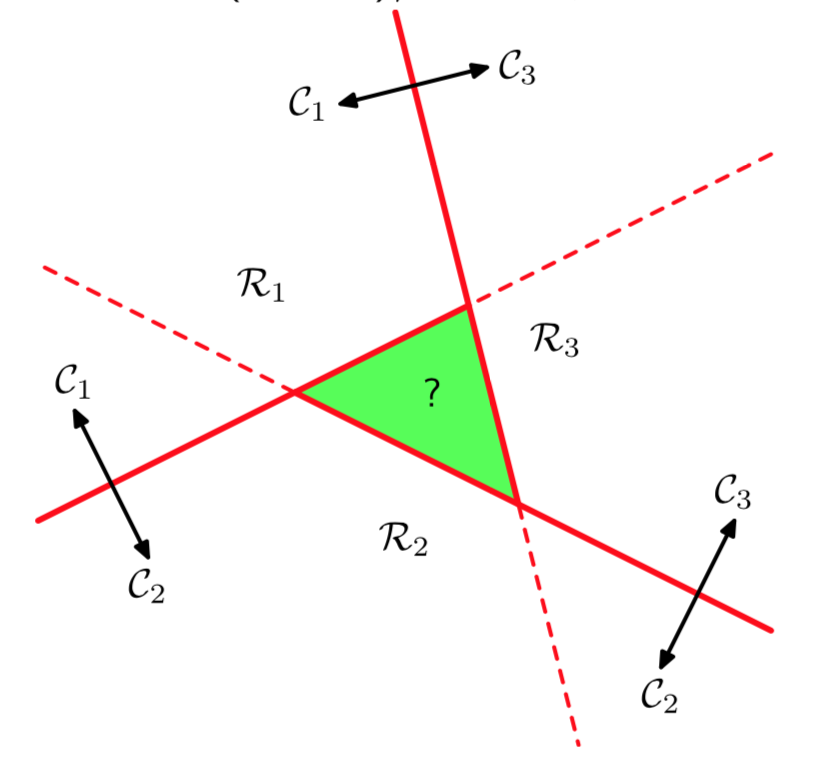
\includegraphics[width=5cm]{ovo_linear.png} }}%
    \qquad
    \subfloat[One Versus Rest]{{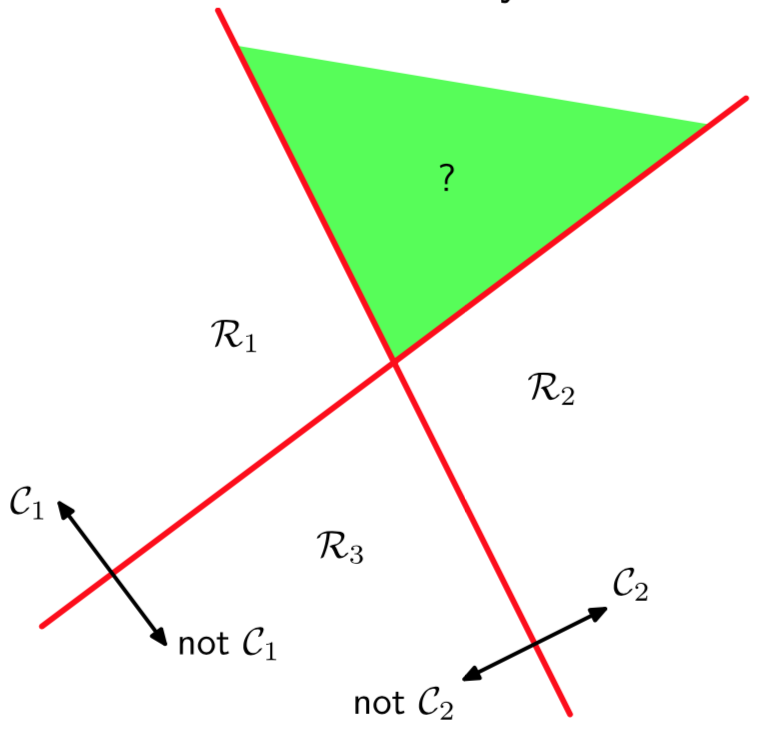
\includegraphics[width=5cm]{ovr_linear.png} }}%

\caption{One Versus Rest }
\label{fig:linear_problem}

\end{figure}


A solution is using a \textbf{K-Class Discriminant}:
\[f: y_k(\bm{x})=\bm{w}_k^T\bm{x}+w_{k0}\]
Where the decision boundary between two classes $C_j,C_k$, is given by:
\[(\bm{w_j}-\bm{w_k})^T\bm{x}+(w_{j0}-w{k0})\]
which can be written in a more compact notation having:
\begin{itemize}
\item $\cmp{w_k}=\binom{w_{k0}}{\bm{w_k}}$
\item $\cmp{x}=\binom{1}{\bm{x}}$
\item $\cmp{W}=(\bm{w_1},\bm{w_2},...\bm{w_k})$
\end{itemize}
We get:
\[\bm{y(x)}=\cmp{W}^T\cmp{x}\]
As shown in figure \ref{fig:k_discriminant}.

\begin{figure}[H]
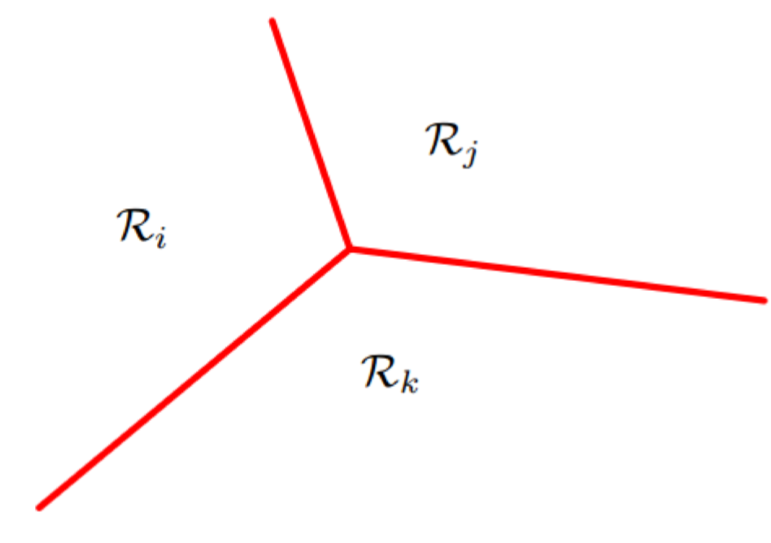
\includegraphics[scale=0.5]{k_discriminant.png}
\caption{K-class discriminant}
\label{fig:k_discriminant}
\end{figure}

Our goal is to determine a good $\cmp{W}$, there are various techniques we can use.

\subsubsection{Least Squares}
Given a dataset $D$ made of instances associated with a one hot vector encoder:
\[\forall x_i \in D: iff\ x_i \in c_k \rightarrow t_i=(0,0,...,1,...0): t_i[k]=1\]
The Least Square aims to minimize the sum-of-square error function


\subsubsection{Fischer linear discriminant}
The main idea is to find projection to a line s.t. samples from different classes are well separated.\\
Suppose we have two classes and $n$ samples $x_1,...,x_n$ where $n_1$ samples are from class $1$ and $n_2$ are from $2$.\\
Considere a line which direction is given by a vector $v$, so that $v^tx_i$ is the projection of a point $x_i$ (2D) onto the line (1D).\\
We have that the mean of the points of classes $1$ is:
\[\mu_1=\frac{1}{n_1}\sum_{x_i \in C_1}^{n_1}x_i\]
Same thing for $\mu_2$. While the mean of the points \textbf{projected} onto the line is simply:
\[\tilde{\mu_1}=v^t\mu_1\]
So we can use $dist=|\tilde{\mu_1} -\tilde{\mu_2}|$ as a measure of separation, since the bigger the better, but look at Figure \ref{fig:fisher1}:

\begin{figure}[H]
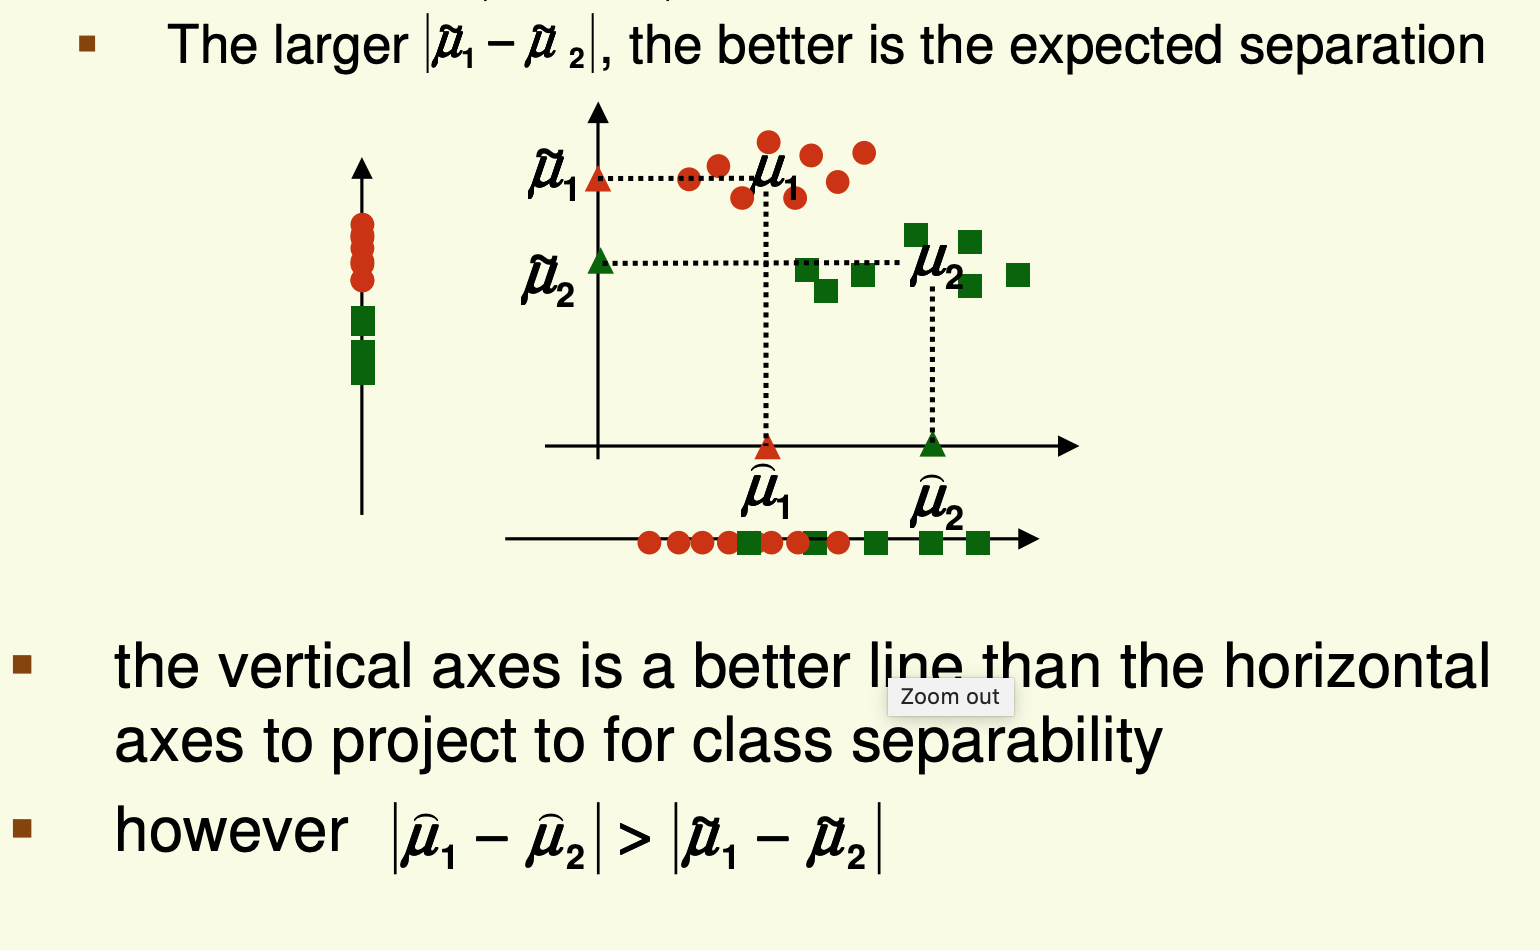
\includegraphics[scale=0.5]{fisher1.png}
\caption{Mean proble}
\label{fig:fisher1}
\end{figure}

The problem is that it does not consider the variance between classes, so we need to normalize $dist$ by something proportional to the variance.\\
Let's define the \textit{scatter} of some samples $z_1,...,z_n$ as :
\[s=\sum_{i=1}^n(z_i-\mu_z)^2\]
Which is:
\[s_1^2=\sum_{x_i \in C_1}(x_i-\tilde{\mu_1})^2\]
and the same for $s_2^2$
So we can now normalize the $dist$ by the scatter, getting the fisher linear discriminant:
\[J(v)=\frac{(\tilde{\mu_1}-\tilde{\mu_2})^2}{s_1^2-s_2^2}\]

\subsubsection{Perceptron}

\begin{figure}[H]
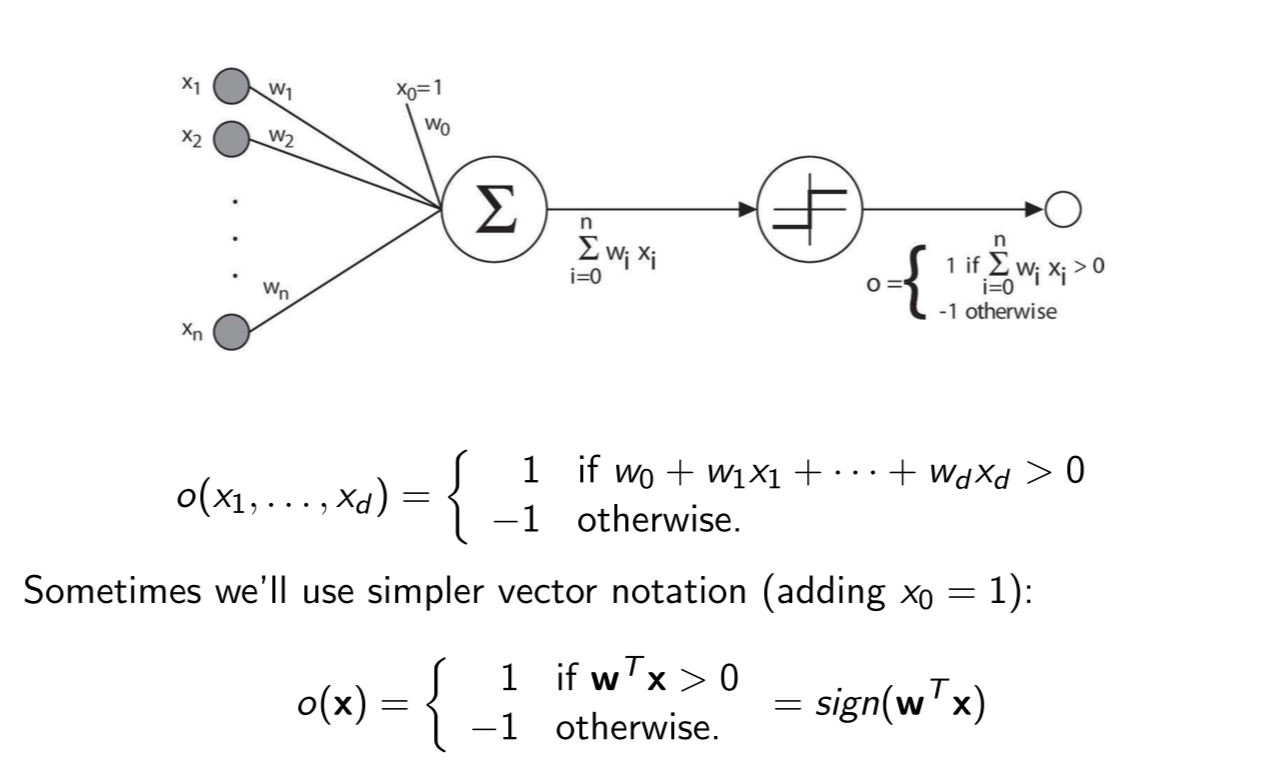
\includegraphics[scale=0.5]{perceptron.png}
\caption{Perceptron}
\label{fig:fisher1}
\end{figure}

The function to minimize is the square error, given the output $o$ and the true label $t$:
\[E(\bm{w})=\frac{1}{2}\sum_{n=1}^N(t_n-o_n)^2=\frac{1}{2}\sum_{n=1}^N(t_n -\bm{w}^Tx_n)^2\]
Since we need to minimize this error we want to move to the direction of the gradient, thus computing the derivative of:
$$\frac{\partial E(\bm{w}) }{\partial w_i}=\sum_{n=1}^N(t_n-\bm{w}^Tx_n)(-x_{i,n})$$
Where $-x_{i,n}$ is the value of i-th feature.\\
so we can update the weight $w_i$ by $w_{i+1}=w_i + \Delta w$, where:

\[\Delta w=-\eta \frac{\partial E(\bm{w}) }{\partial w_i}=\sum_{n=1}^N(t_n-sign(\bm{w}^Tx_n)))-x_{i,n} \]

\begin{figure}[H]
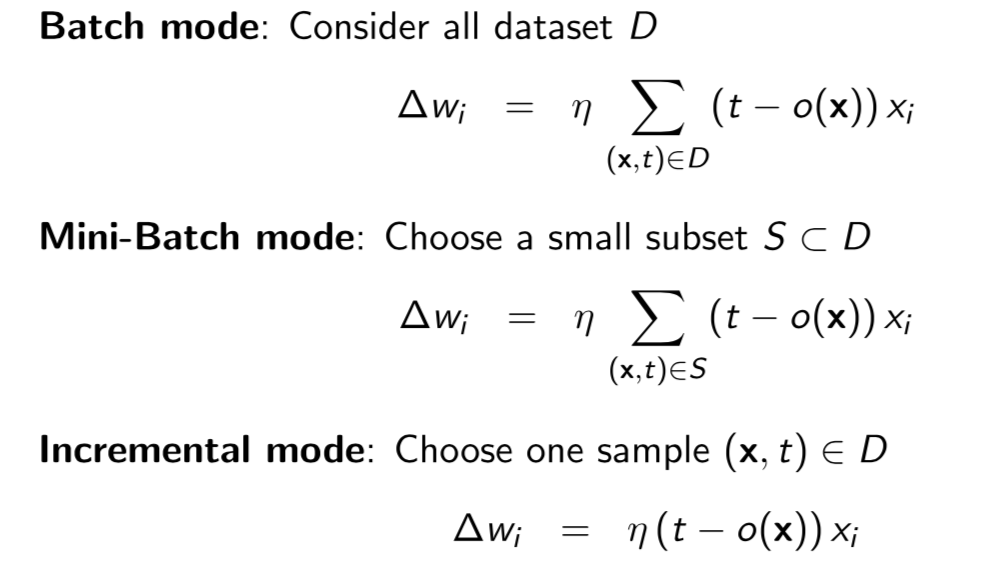
\includegraphics[scale=0.5]{perce_algh.png}
\caption{Perceptron Algotithm}
\end{figure}

\subsubsection{Support Vector Machine [SVM]}
SVMs are based on the idea of finding a hyperplane that best divides a dataset into two classes


\begin{figure}[H]
    \centering
    \subfloat{{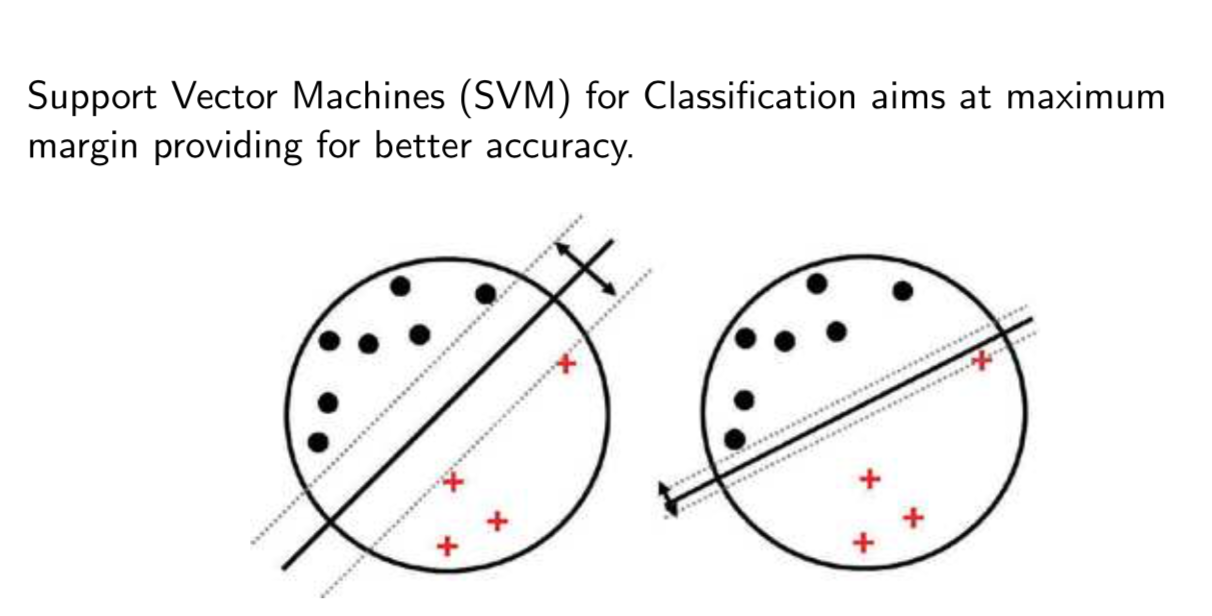
\includegraphics[scale=0.5]{svm1.png} }}%
    \qquad
    \subfloat{{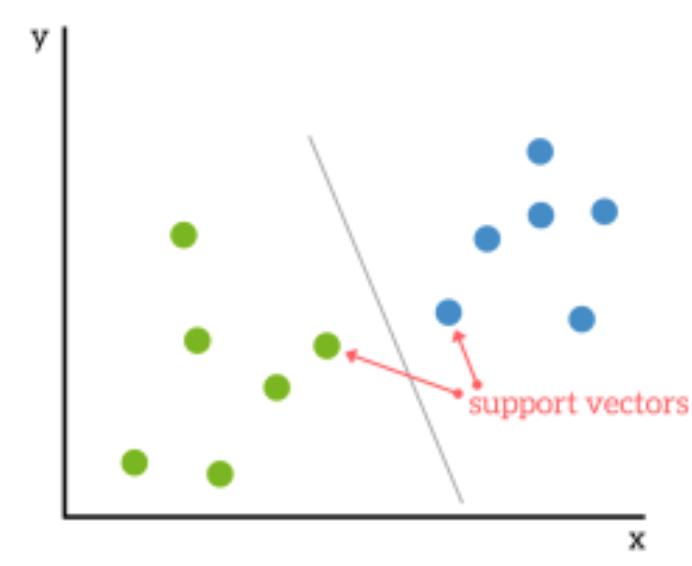
\includegraphics[scale=0.5]{svm2.png} }}%

\label{fig:linear_problem}%
\end{figure}

Support vectors are the data points nearest to the hyperplane, the points of a data set that, if removed, would alter the position of the dividing hyperplane.\\
The distance between the hyperplane and the nearest data point from either set is known as the margin. The goal is to choose a hyperplane with the greatest possible margin between the hyperplane and any point within the training set, where the margin is estimated as:
\[\argmax_{\bm{w},w_0}\frac{1}{||\bm{w}||}\min_{n=1..N}[t_n(\bm{\hat{w}^Tx_n+\hat{w_0}})]\]
Where the
\begin{itemize}
\item $\hat{h}=\bm{\hat{w}^Tx_n+\hat{w_0}}$ is the hyperplane
\item $\frac{1}{||\bm{w}||}\min_{n=1..N}[t_n(\bm{\hat{w}^Tx_n+\hat{w_0}})]$ is the smallest distance between the hyperplane and $x$.

\end{itemize}

\subsection{Regression}
In this case we want to predict a real value function, our model will be of the kind:
$$y(x;w)=W^TX$$
Where both $W,X$ are vectors of dimension $d$.\\
There are some cases in which the dataset is non linear, so we can use a non linear function on $x$ of the kind:
$$y(x;w)=W^T\phi (X)$$
The function could be anything (e.g. $\phi(x)=x^2$) but we still have a linearity in the parameters $W$.

\paragraph{Maximum Likelihood}
If our target value $t$ is affected by noise $\eta$:
$$t=y(X;W)+\eta$$
We now have a probability that the target is correct given the regression. If we assume $\eta$ to be gaussian we have:
$$P(t|X,W,\beta)=N(t|y(X;W),\beta^{-1})$$
Where $\beta$ is the inverse of the variance.\\
The only thing left is to seek that $t \in S$ which maximize this probability:
\begin{equation}
\begin{aligned}
P(S|X,W,\beta)=\prod_n N(t_n|w^T\phi(x_n),\beta^{-1})=\\
\sum_n ln[N(t_n|w^T\phi(x_n),\beta^{-1})]=\\
-\beta \frac{1}{2}\sum_n[t_n-w^T \phi(x_n)]^2-\frac{N}{2}ln[2\pi\beta^{-1})
\end{aligned}
\end{equation}
 
Since the second term is a constant we focus on the first one:
$$E_D(w)= \frac{1}{2}\sum_n[t_n-w^T \phi(x_n)]^2$$
Which we want to minimize.

\paragraph{Regularization}
To control overfitting we can set a regularization factor on the parameters of the kind:
$$E_W(w)=\frac{1}{2}W^TW$$
So that the minimization becomes:
$$min[E_D(w)+\lambda E_W(w)]$$



\newpage



\section{Probabilistic Generative Models}
Consider the case of two classes $C_1,C_2$, we have that:
\[P(C_1|x)=\frac{P(x|C_1)P(C_1)}{P(x|C_1)P(C_1)+P(x|C_2)P(C_2)}\]
with:
\[\alpha=ln\frac{P(x|C_1)P(C_1)}{P(x|C_2)P(C_2)}\]
We can write:
\[\sigma(\alpha)=\frac{1}{1+exp(\alpha)}\]
Which is the sigmoid function.

\newpage
\section{Multiple Learner}
The idea is : instead of training a complex learner/model, train many different learners/models and then combine their results.

\paragraph{Voting}
Here the models are trained in parallel on the same dataset $D$ and then take the outputs are summed (for regression) or chosen based on the most voted class (for classification).

\paragraph{Bagging}
In here he separate the dataset $D$ into $M$ parts (called bootstraps), then we train a different learner for each part and average the results.

\subsection{Boosting}
Contrary to the other methods, the boosting train weak classifiers sequentially. This is because some weak learner at iteration $i$ will output a miss-classified $y_{i,n} \ne t_n$ associated with a point $x_n$ and its weight $w_{i,n}$ . During the next training iteration the learner will find the weight associated with the point $x_n$  greater than it was before $w_{i+1,n} >w_{i,n}$ so that this learner learns to give more importance tho this point and avoid future miss-classifications.

\paragraph{AdaBoost}
AdaBoost works as just described using decision trees with a signle split.\\

The advantages are:
\begin{itemize}
\item fast, simple
\item no prior  about base learner
\item no parameter to tune
\item can be combined with any method
\end{itemize}

 The algorithm works as follows:
\begin{enumerate}
\item having a Dataset $D$ of size $N$ you want to train $M$ learners. Each one will have its own weight array $w_m$ of size $N$ (one value for each data point)
\item Initialize all the weights to  $w_m=1/N$.
\item Start from the first learner until the last one $M$ and do:
\item Train the learner minimizing the weighted error function :
$$J_m=\sum_n w_{m,n}I(e)$$
Where $e=y_m(x_n) \ne t_n \in \{0,1\}$ is the correctness of the classification
\item Evaluate the error for this classifier as:
$$\eta_m=\frac{J_m}{w_m},\quad \alpha_m=ln[\frac{1-\eta_m}{\eta_m}]$$
Where $\alpha_m$ will be used later to estimate the grade of correctness

\item Generate the weight for the next learner $m+1$ as:
$$w_{m+1,n}=w_{m,n}\cdot \exp[\alpha_m I(e)]$$
\end{enumerate}
As can be seen the next weight $w_{m+1,n}$ associate with a specific datapoint $x_n$ will be updated by $\alpha_m$ iff the classification is incorrect $ I(e)=0\ if\ y_m(x_n) = t_n$.


\newpage
\section{MDP and RL}
In a dynamic system representation we have:
\begin{itemize}
\item A set of states $X$
\item A set of actions $A$
\item a transition function $\delta$  which can be 
\begin{itemize}
\item deterministic $\delta : X\times A \to X$
\item non deterministic $\delta : X\times A \to 2^X$
\item stochastic $\delta : P(x_{t+1}|x_t,a_t)$
\end{itemize}
\item A reward function $r$ which can be:
\begin{itemize}
\item deterministic $r: X \times A \to R$
\item non deterministic $r: X \times A \times X \to R$
\end{itemize}
\end{itemize}

\paragraph{Markov decision process}
A MDP follows the Markov properties which state:
\begin{itemize}
\item Once the current state is known, the evolution of the dynamic system does not depend on the history of states, actions and observations $x_{t+1}=\delta(x_t,a_t)$.
\item The current state contains all the information needed to predict the future.
\item Future states are conditionally independent of past states and past observations given the current state.
\item The knowledge about the current state makes past, present and future observations statistically independent.
\end{itemize}

\paragraph{Policy}
A policy $\pi$ is some kind of behavior that takes as input some state $x_t$ and chooses an action $a_t$  in order to maximize the reward $r_t$.\\
The optimality of a reward is defined with respect to maximizing the (expected value of the) cumulative discounted reward:
$$V^{\pi}(x_1)=E[r_1+\gamma r_2+\gamma^2 r_3+\dots]$$
Where $\gamma \in [0,1]$ is the discount factor.

\subsection{RL}
Missing

\newpage
\section{HMM and POMDW}
If the states $x$ of a markov process are non-observable, but instead we have some observation $z$ tied to them we are dealing with a Hidden Markov Model [HMM].\\
In this case the process is defined by:
\begin{itemize}
\item The \textbf{observation model}: a probability that a certain state is mapped with a specific observation $b_k(z_t)=P(z_t|x_t)$ 
\item The \textbf{transition model}: $A_{ij}=P(x_t|x_{t-1})$
\item an initial distribution $\pi_0=P(x_0)$ which define the probability that the model starts with the state $x_0$
\end{itemize}

\paragraph{Chain Rule}
Since we are dealing with a model having the markov assumption (current observation only depends on past $N$ observation) we can extend this rule to apply to a series of state/obervation pair:
$$ P(x_{0:T},z_{0:T})=\prod_{t=1}^Tp(z_t|x_t) \prod_{t=1}^Tp(x_t,x_{t-1})$$

\paragraph{Forward Pass}
So now we have a sequence of observation $z_0,z_1,\dots,z_T=[z]_{t=1}^T$ and we would like to know how likely this sequence is $P([z]_{t=1}^T)$.\\
This probability  requires summing over \textbf{all possible hidden state values} at all times:
\begin{equation}
\begin{aligned}
P([z]_{t=1}^T)=p(z_0,z_1,\dots, z_T; x_0,x_1,\dots,x_T)+p(z_0,z_1,\dots, z_T; x_1,x_2,\dots,x_T)+\dots\\
+p(z_0,z_1,\dots, z_T; x_{T-1})+p(z_0,z_1,\dots, z_T; x_T)=\sum_{n=0}^Np([z]_{t=1}^T,[x_n]_{t=1}^T)
\end{aligned}
\end{equation}

Considering the first term we can apply the chain rule to get :
$$p(z_0,z_1,\dots, z_T; x_0,x_1,\dots,x_T)=P(z_{0:T};x_{0:T})=\prod_{t=1}^Tp(z_t|x_t) \prod_{t=1}^Tp(x_t,x_{t-1})$$
So the previous equation becomes:
 $$P([z]_{t=1}^T)=\sum_{n=0}^Np([z]_{t=1}^T,[x_n]_{t=1}^T=\sum_{n=0}^N P(x_0)\prod_{t=1}^Tp(z_t|x_t) \prod_{t=1}^Tp(x_t,x_{t-1})$$
 Which is a lot of calculation to do!\\
 
 But if we set  $p([z]_{t=1}^T,x=k)=\alpha_T^k$ we can rewrite the above equation as:
 $$P([z]_{t=1}^T)=\sum_k\alpha_T^k$$
 Which gives the forward step as:
 \begin{enumerate}
 \item Initialize $\alpha_1^k=P(z_1|x_1=k)p(x_1=k)$ for all k
 \item for $t=2,\dots,T$ estimate 
 $$a_t^k=p(z_t|x_t=k)\sum_i \alpha_{t-1}^ip(x_t=k|x_{t=1}=i)$$
 \item terminate when 
 $$P([z]_{t=1}^T)=\sum_k\alpha^k_t$$
  \end{enumerate}

 \paragraph{Backward step}
 Now we want to find the probability that the hidden state $x$ at time $t$ was equal to $k$:
 $$P(x_t=k|[z]_{t=1}^T)=P(z_1,\dots,z_t,x_t=k)P(z_{t+1},\dots,z_T|x_t=K)=\alpha^k_t\beta_t^k$$
 So now we compute the backward algo with:
 \begin{enumerate}
 \item initialize $\beta_T^k=1$ for all $k$
 \item for $t=T-1,\dots,t$ do:
 $$\beta_t^k=\sum_i P(x_{t+1}=1|x_t=k)P(z_{t+1}|z_{t+1}=i)\beta^i_{t+1}$$
 \item ternimate at:
 $$P(x_t=k,[z]_{t=1}^T)=\alpha^k_t\beta^k_t$$
 \end{enumerate}
 
 \subsection{POMDP}
 In a Partially Obervable MDP we cannot see the states, so we can use a belief $b(x)$ which is a probability distribution over the states.\\
 Given a current belief state $b$, an action $a$ and an observation $z'$, we want to compute the next belief state $b'(x')$:
 $$b'(x')=P(x'|b,a,z')=\frac{P(z'|x'b,a)P(x'|b,a}{P(z'|b,a)}=\frac{P(z'|x',a)\sum_{x\in X}P(x'|b,a,x)P(x|b,a)}{P(z'|b,a)}$$
 

 

\newpage
\section{Non-deterministic RL}
When the problem is non deterministic we know that the transition function $\delta(x,a)$ is some probability related to the current state and action $P(x_{i+1}|x_i,a_i)$.\\

To define our value function, we must take the expected values:
$$V^{\pi}(x)\equiv E(r_i +\gamma r_{i+1}+\gamma^2 r_{i+2}+ \dots)$$

When we consider the reward function, $r(x,a)$, to be non deterministic too, then we must include it in the value function which we now call $Q$:
$$Q(x,a)=E[r(x,a)+\gamma V^*(\delta(x,a))]=\dots=E[r(x,a)]+\gamma \sum_{x_{i+1}}P(x_{i+1}|x_i,a)\cdot \max_{a_{i+1}}Q(x_{i+1},a_{i+1})$$
Where:
\begin{itemize}
\item $E[r(x,a)]$ is the expected reward
\item $P(x_{i+1}|x_i,a)$ is the probability introduced above with the transition function
\item $\max_{a_{i+1}}Q(x_{i+1},a_{i+1})$ is finding the action which maximizes the future rewards
\end{itemize}
Where now the optimal policy shift to:
$$\argmax_{a\in A}Q(x,a)$$

\subsection{K-Armed bandit problem}
The classic (stocastic) version of the k-armed bandit problem sees k slot machines, each one having some gaussian distribution of winning $N(\mu_i,\sigma_i)$ and the goal is to earn the most money.\\
In this context a RL agent can either:
\begin{itemize}
\item Perform x trials on each machine, estimate the mean winning rate and then choose the one with the highest.
\item Adopt an $\epsilon$-greedy strategy in which they play at random with prob $\epsilon$ and choose the optimal policy with $1-\epsilon$
\end{itemize}

In this case the training rule would be:
$$Q_n(a_i) \leftarrow Q_{n-1}(a_i)+ \alpha[r_{t+1}(a_i) - Q_{n-1}(a_i)]$$
Where 
\begin{itemize}
\item $\alpha=1/v_{n-1}(x_i,a_i)$
\item $v_{n-1}(x_i,a_i)$ is the number of execution of action $a_i$ in state $x_i$, up to time $n-1$
\end{itemize} 

\paragraph{Non-deterministic case}
But if the probability $\mu_i$ changes during the algorithm then the above solution would not work:
\begin{itemize}
\item the first would fail because $\mu_i$ can change after the $x$ trials
\item the $\epsilon$-greedy strategy will not reach an optimal value
\end{itemize}


\newpage
\section{Dimensionality Reduction}

\paragraph{Latent Variable}
Usually, in a dataset with  high dimensional data, the difference between the samples can be related to a distortion regarding fewer dimensions than the ones making up the sample itself. For example, in a 2D image undergoing a one degree of freedom rotation the latent variable would be $1 < 2$.\\

\subsection{PCA} 
Check out \hyperlink{https://www.youtube.com/watch?v=FgakZw6K1QQ}{this video} for a detailed explanation of PCA.\\

\paragraph{Steps}
The main goal of PCA is to find a line $u$ which best separates the projected points $x$ of the dataset. To find this line we need to :
\begin{enumerate}
\item Find the mean value of all the points $x=\hat{x}=\frac{1}{N}\sum_nx_n$
\item Estimate the total variance as $S=\frac{1}{N}\sum_n(x_n-\hat{x})(x_n-\hat{x})^T$
\item Maximize the projected variance $\max_{u}[u^TSu]$ 
\end{enumerate}

\paragraph{Solution}
To find $u$ we derivate wrt $u$:
$$S u=\lambda u \to u^TSu=\lambda$$
Which means that $u$ must be the eigenvector of $S$ since $\lambda$ is its eigenvalue.\\
So having the matrix $S$ the easiest thing is to find the eigenvector associated with the largest eigenvalue.

\paragraph{Error Minimization}
With the above solution we can rewrite some sample $x$ of dimension $D$ as $\tilde{x}$ of dimension $\tilde{D}<D$. This will inevitably lead to some error which we can estimate with:
$$J=\frac{1}{N}\sum_n ||x_n-\tilde{x}_n||^2=\sum_{i=\tilde{D}+1}^D u_i^T S u_i=\sum_{i=\tilde{D}+1}^D \lambda_i$$
So the error is the sum of all the discarded eigenvalues $\lambda_i$ after $\tilde{D}$.

\subsection{Linear Latent Variable Model}
How to estimate PCA efficently?

\paragraph{Distributions}
For this we assume that:
\begin{itemize}
\item The relationship between $x$ and its lower dimensional representation $\tilde{x}$ is linear and can be written as:
$$x=W\tilde{x}+\mu$$
\item $\tilde{x}$ has a gaussian distribution of the form $P(\tilde{x})=N(z,0,I)$
\item The relationship between $x$ and $\tilde{x}$ is linear in the Gaussian space:
$$P(x|\tilde{x})=N(x,W\tilde{x}+\mu,\sigma^2 I)$$
\end{itemize}

Then we have:
\begin{itemize}
\item Marginal Distribution $P(x)=N(x, \mu, C)$
\item Posterior Distribution $P(\tilde{x}|X)=N(\tilde{x},M^{-1}W^T(x-\mu),\sigma^2 M)$
\item $C=WW^T+\sigma^2I$
\item $M=W^TW+\sigma^2I$
\end{itemize}

\paragraph{Maximum Likelihood}
Since we have $P(x)$ and $P(\tilde{x}|X)$ we can use ML to estimate $W$ which depends on the $u$ as:
$$\argmax_{W,\mu,\sigma}[ln P(X|W,\mu,\sigma^2)]$$

\subsection{Autoencoders}

These are NN with bottolnecks in the middle which learn to reconstruct their input by minimizing a sum-of-squares error.

\paragraph{Generative}
This kind of autoencoders focus on leargning the latent space structure.\\
VAEs are an example which use an encoder to produce  a distribution and a decoder to produce sample from such distribution.\\
Since the sampling operation is not differentiable they use a reparametrization 

\paragraph{Generative}
This kind focus on learning the distribution.\\
GANs are an example which are basically an inverted CNN trained in an adversarial way 



\newpage
\section{Kernel}
Kernels are just a type of similarity measures which can be applied in any circumstance. Since they are a similarity measure they take as input two variables and return a value:
$$k(x_1,x_2)\in R$$
Typically they are simmetric $k(x_1,x_2)=k(x_2,x_1)$ and non negative.

\paragraph{Gram Matrix}
Given a  linear model of the form $y(x,w)=w^tx$ we know that the optimal solution is given by :
$$w*=X^T(XX^T+\lambda I)^{-1}t$$
Where $X,t$ are the vector of samples and outputs.\\
By setting $\alpha=(XX^T+\lambda I)^{-1}t$ we get:
$$w*=X^T\alpha=\sum_n\alpha_nx_n$$
So the linear model becomes:
$$y(x,w)=w*^Tx=\sum_n\alpha_nx^T_nx$$
As can be seen the last equation has two inputs $x_n,x$ so we can use a kernel $k(x_1,x_2)=x_1^Tx_2$ to get the same result:
$$y(x,w)=w*^Tx=\sum_n\alpha_n k(x_n,x)$$
If we now look into $\alpha$ we see that the term $XX^T$ (which we will  call $K$) can be also kernelized as:
$$K=
\begin{bmatrix}
k(x_1,x_1) & \dots & k(x_1,x_N)\\
\vdots & \ddots & \vdots\\
k(x_1Nx_1) & \dots & k(x_N,x_N)\\
\end{bmatrix}
$$
Which is called the Gram matrix.

\paragraph{Kernel Trick}
The thing we did above, substituting the inner producct $X^TX$ with the kernel $k(x^T,x)$ is called the kernel trick and can be applied to any $x$. But why is it useful?\\
Having a linear model of the kind :
$$y(x,w)=w*^Tx=\sum_n\alpha_nx^T_nx$$
Shows that we actually do not need to know each datapoint but just its inner product $x^Tx$. So if our dataset is linearly separable in a higher dimension we do not need to compute the projection of each point $x_i$ into that higher dimension, but we just need to compute the inner product in that dimension. So we can use the kernel trick to get that product and ease the computation.



\newpage
\section{Artificial Neural Network}

\subsection{FeedForward NN}

There are no loops in this NN, the final function is a composition of multiple functions $g$ and parameters $\theta$ (one for each layer $m$):
$$f(X,\theta)=g_m(g_{m-1}(\dots(g_1(x,\theta_1)\dots)\theta_{m-1})\theta_m)$$
These many functions can tackle non-convex problems contrary to linear or kernel methods.\\

\paragraph{Depth}
The depth of a FNN is given by the number of hidden layers. With enough hidden layer you can  approximate any Borel measurable function.

\paragraph{Width}
Is the number of units (neurons) in each layer, with enough units you can approximate any function but having a deeper FNN is easier to train.



\paragraph{Output activation Functions}
These functions are tied to the output of the FNN, so they are dependent of the problem at hand and shape the cost function. Since they come after the hidden unit output $h_i$, they will show such parameter in their input.\\
They change together with the problem requirement:
\begin{itemize}
\item Regression: we use the identity function: $y=W^th+b$
\item Binary classification: sigmoid is used: $y=\sigma(w^th+b)$
\item  Multi-class classification= softmax: $y_i=softmax(\alpha)_i=\frac{e^\alpha_i}{\sum_j e^\alpha_j}$
\end{itemize}


\paragraph{Loss Functions}
The loss function is the cost function used for training. The value of such functions is simply the natural logarithm $ln$  of the output activation function.\\
Recall the ML in which we wanted the class which maximized $P(C_i|x,D)$, if we use the same principle here we get the \textbf{cross-entropy} loss function:
$$J(\theta)=-ln(P(t|x,\theta))$$

Which changes depending on the problem at hand,   In the following cases $\alpha=w^th+b$
\begin{itemize}
\item Regression: then $P(t|x)=N(t|y,\beta^{-1})\to J(\theta)=(t-f(x,\theta))^2/2$ so the cost function becomes the mean square error.
\item Binary classification: $J(\theta)=softplus((1-2t)\alpha$ becomes a Bernoulli Distribution
\item Multi-class classification= $J(\theta)_1=-ln\ softmax(\alpha)_1$ becomes a Multinomial distribution.
\end{itemize}

\paragraph{Hidden activation functions}
In this case the activation function can be diverse for each neuron.
\begin{itemize}
\item Rectified linear units (ReLU): $g(\alpha=max(0,\alpha$ which is easy to optimize but not differentiable at 0.
\item Sigmoid $g(\alpha)=\sigma(\alpha)$ and hyper tan $g(\alpha)=thanh(\alpha)$, both are:
	\begin{itemize}
	\item Easy to saturate since there is no logarithm at the output
	\item slow
	\item usefull for RNN and autoencoders
	\end{itemize}
\end{itemize}

\paragraph{Backprop}
Since the error is estimated at the end of the FNN on the outputlayer, but he have multiple parameters $\theta$ which need to be updated, we must propagate the error back trough the network.\\
For this reason we compute the gradient of the cost function with respect to each parameter using the chain rule which states that, having $z=f(g(x))$ (similar to a network having one hidden layer) the gradient of z with respect to x is:
$$\frac{dz}{dx}=\frac{dz}{dy}\frac{dy}{dx}$$

\subsection{Learning Algorithms}
Since the backprop is just a method to compute the gradient (not learn) there are various other algo for this purpose.

\paragraph{Stocastic Gradient Descent}
Using a learning rate $\eta$ these method computes the gradient on a subset (minibatch) of samples from the dataset. This gradient is computed with the backprop method and the parameters are updated with the following formula:
$$\theta_i^{(k+1)}=\theta_i^{(k)}-\eta g_i$$
Where $g$ is the value of the gradent with respect to $\theta_i$.

\paragraph{SGD with momentum}
To speed up the training an additional parameter $v$ can be used to increase or decrease the value of the update depending on the training iteration.

\subsection{Regularization}
Reduces overfitting

\paragraph{Parameter norm penalties}
You can add a regularizatoin term to the cost function in order to decrease the magnitude of each parameter, so no parameter saturates.

\paragraph{Dataset Augmentation}
Transform the dataset (image distortion, noise adding) in order to have more diverse samples.

\paragraph{Early stopping}
Stop iteration to avoid overfitting when train loss zeros out while test loss increases.

\paragraph{Parameter sharing}
Constrain subset of parameters to be the same. Decrease memory consumption, used principally in CNN to allow translation invariance.

\paragraph{Dropout}
Randomly remove network units with some probability.


\newpage
\section{CNN}
In CNNs there are usually three stages:
\begin{enumerate}
\item Convolution: in which the dimension of the input is reduced and the most important features are extracted
\item Activation function: usually non linear, allows the method to apply to non linearly separable datasets
\item Pooling: an averaging of some sort (usually max or average) used to implement invariance to local translations. If applied with a stride $\ge 0$ then it reduces the dimension of the output.
\end{enumerate}

Since the convolution is done with a kernel (which can be seen as a rectangle taking as input some pixels and outputting one) of size $k$ the parameters become $k$ instead of $m \times n$ which is the size of the network. But since the kernel requires the input to have a certain dimension (to be applied to the borders too) we need to pad the images on the borders.

\paragraph{Number of Parameters}
The number of parameters of a layer $i$ depends on the previous output $i-1$ and the kernel size.\\
With images of size $k \times  v \times d$ the third dimension $d$ is the feature map (in 2D dataset it's considered to be 1), a conv layer $i$ takes as input some data with $x_i$ feature map and outputs $y_i$ feature maps.\\
Having a kernel of size $n \times m$ the parameters of layer $i$ are :
$$|\theta_i|=(n\times m\times x_i +1)\times y_i$$
It is trivial to see that the parameters are much less than in the FCN where we have:
$$|\theta_i|=(k +1 ) \times v$$
Usually $ k \gg n$ and $v \gg m$.

\paragraph{Output Dimension}
Here we want to know what is the dimension of the output of a conv layer. For this we need two additional parameters which are the padding $p$ and the stride $s$. The output is of dimension $w_i \times h_i \times d_i$ where $d$ is also called the feature map.\\
The dimensions depend on the previous ones as follows:
\begin{equation}
\begin{aligned}
w_i=\frac{w_{i-1}-n+2p}{s}+1\\
h_i=\frac{h_{i-1}-m+2p}{s}+1\\
d=d_i
\end{aligned}
\end{equation}

\newpage
\section{Unsupervised}
This kind of learning is used when a dataset does not have any label $t$, so we need to cluster similar samples $x$ based of some other metrics.

\subsection{Gaussian Mixture Models }
One way is to assume the data is made of a mixture (sum) of gaussians , so we let the model maximize the probability of  \textit{K} gaussians.\\
This model will have three parameters for each $k$:
\begin{itemize}
\item a mean $\mu$
\item a co/variance $\Sigma$
\item a mixing probability $\pi$ that defines how big or small the Gaussian function will be. 
\end{itemize}
Obviously the total mixing probability should sum up to 1 $\sum_k \pi_k=1$.\\
Normally, for one Gaussian, we would use ML and differentiate on $\mu, \Sigma$ to get the optimal weight value, but here we are dealing with multiple Gaussians which may render this approach unfeasible.

\paragraph{Latent variable}

So now, for each gaussian $k$, we assocaite a (latent) variable $z_k$ to it and say that if a datapoint $x_n$ is coming from that specific gaussian then $z_k=1$. So the probability  that a data point $x_n$ comes from Gaussian $k$ is:
$$P(z_{n,k}=1|x_n)$$
It is trivial to see that the bigger the gaussian is (bigger $\pi_k$) the more likely is that a datapoint $x_n$ belongs to it, so:
$$\pi_k=p(z_k=1)$$
That is the  overall probability of observing a point that comes from Gaussian \textit{k} is actually equivalent to the mixing coefficient for that Gaussian.\\
If we consider all the statistically independent (latent) variables $Z=z_1,z_2,\dots, z_K$, the probability would be:
$$p(Z)=\prod_k \pi_k^{z_k}$$

\paragraph{Joint Distributions}
We still wish to find the probability that a point $x_n$ belongs to some gaussian $k$, we can do so with:
$$p(x_n|z)=\prod_k N(x_n|\mu_k,\Sigma_k)^{z_k}$$
By applying the chain rule we know that:
$$p(x_n,z)=p(x_n|z)p(z) \to p(x_n)=\sum_k p(x_n|z)p(z)= \sum_k \pi_k N(x_n|\mu_k,\Sigma_k)$$
Finally we  can find the likelihood as the joint probability of all observations $x_n$, defined by:
$$p(X)=\prod_n  p(x_n)=\prod_n \sum_k \pi_k N(x_n|\mu_k,\Sigma_k)$$

\paragraph{Expectation Maximization}
Let's define :
$$\gamma(z_k) \equiv P(z_k=1|X)=\frac{P(z_k=1)P(X|z_k=1)}{P(X)}=\frac{\pi_k N(X;\mu_k,\Sigma_k)}{\sum_j^K \pi_j N(X;\mu_j,\Sigma_j)}$$
We need to determine $\mu_k, \Sigma_k, \pi_k$.\\
Using ML we get:
\begin{itemize}
\item $\mu_k=\frac{1}{N_k}\sum_n \gamma(z_{nk})x_n$
\item $\mu_k=\frac{1}{N_k}\sum_n \gamma(z_{nk})(x_n-\mu_k)(x_n-\mu_k)^T$
\item $\pi_k=\frac{N}{N_k}$
\item $N_k=\sum_n\gamma(z_{nk})$
\end{itemize}

The steps for the algorithm are reported in the next figure.

\begin{figure}[H]
\centering
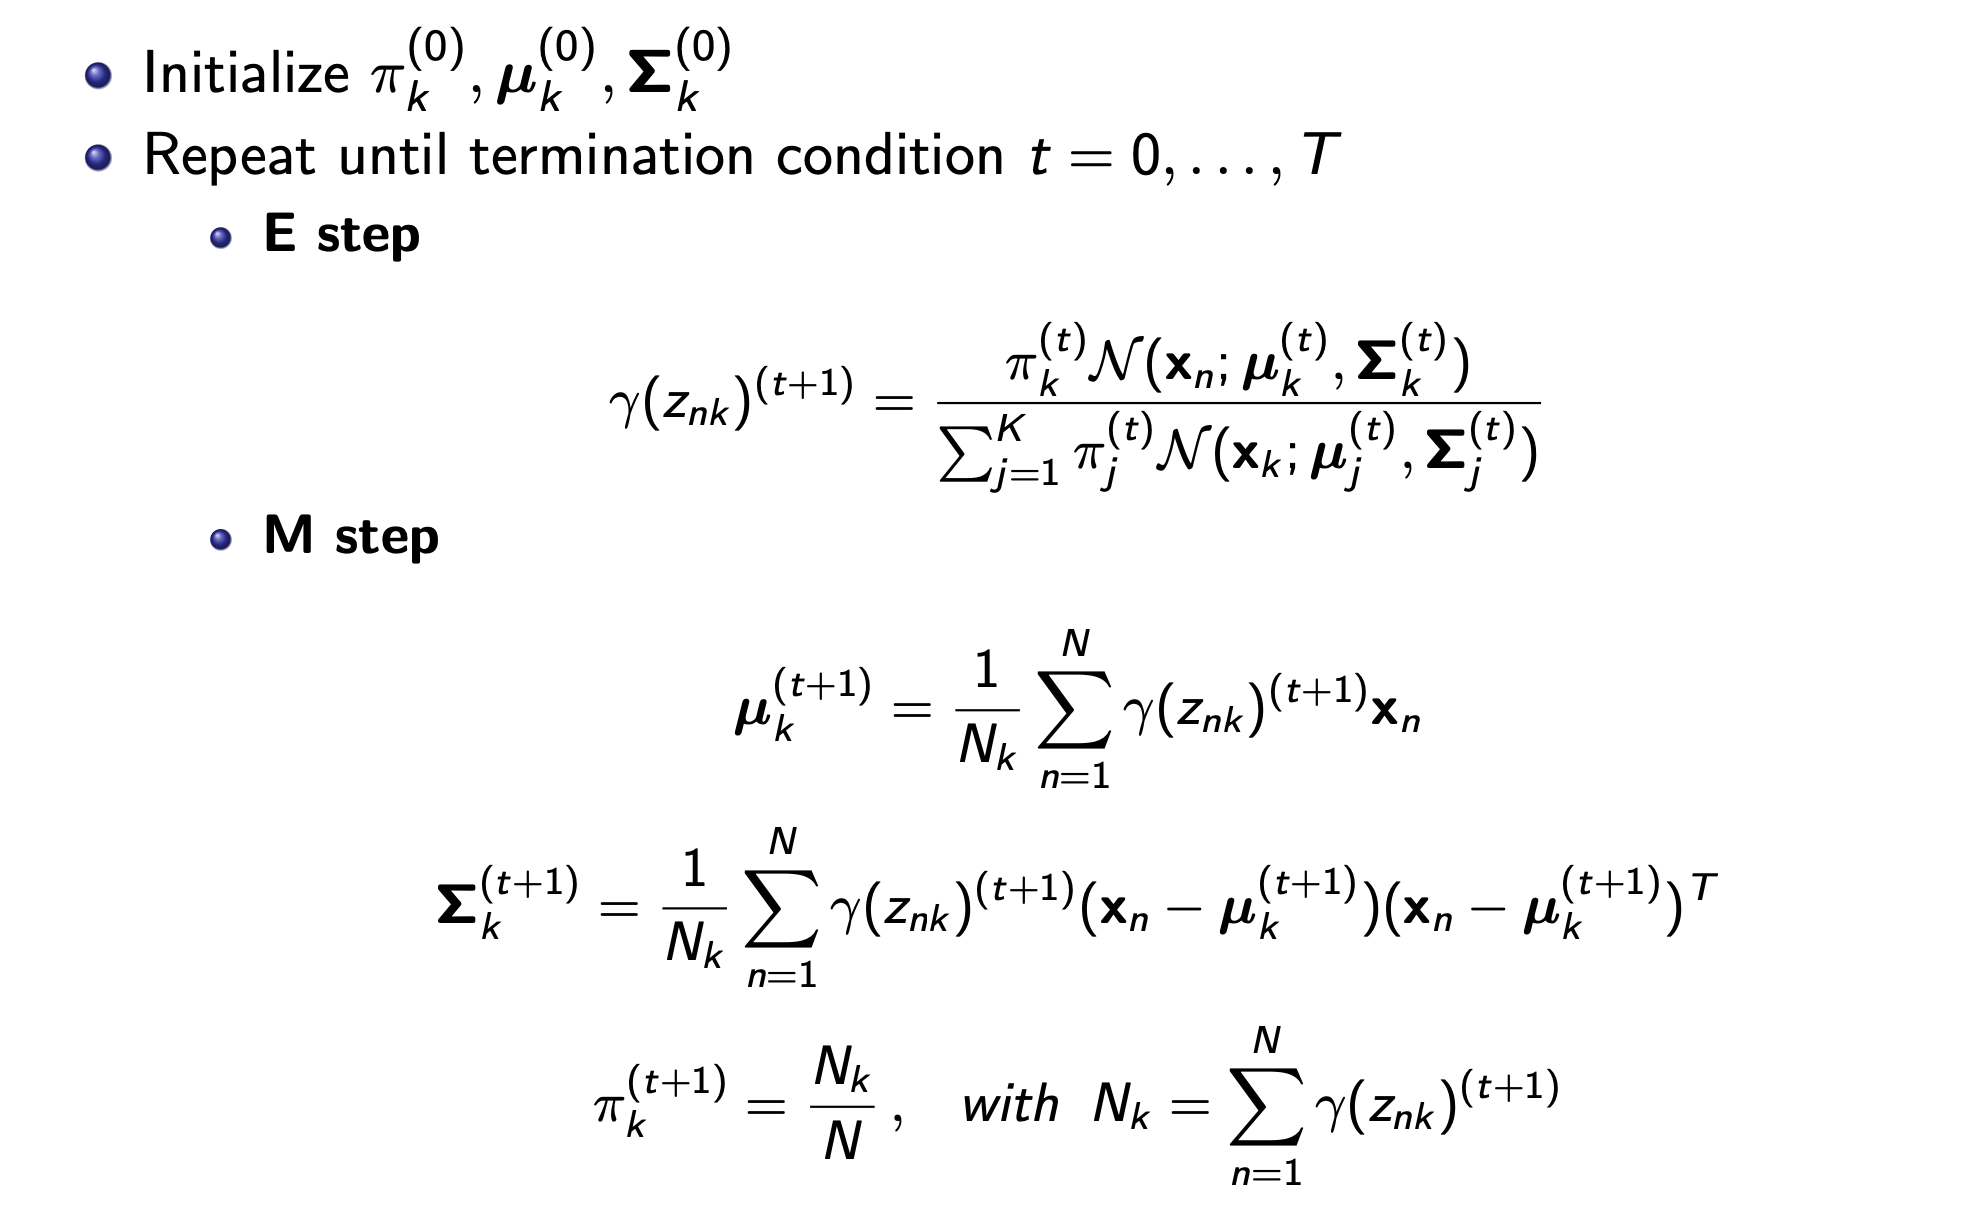
\includegraphics[scale=0.3]{gmm_em}
\end{figure}

\subsection{K-means}
In this one you first decide the number of clusters $K$. The you start the algorithm:
\begin{enumerate}
\item Partition the dataset into $K$ parts at random or use some kind of initialization algorithm
\item For each partition estimate the centroid $c_i=\frac{1}{N_k}\sum_k x_k$ 
\item For each sample $x$, compute two distances:
\begin{itemize}
\item Distance $d_i$ between $x$ and its current centroid $c_i$ 
\item Distance $d_{j}$ between the $x$ and the closest centroid $c_j$.
\end{itemize}
\item if $d_j<d_i$ assign $x$ to $d_j$
\item repeat until convergence
\end{enumerate}

\paragraph{Convergence}
Convergence is achieved if:
\begin{itemize}
\item The number of clusters $K$ is finite
\item $d_i$ decreases at each iteration 
\end{itemize}

\paragraph{Cons}
\begin{itemize}
\item K must be determined before hand
\item Sensitive to initial condition (local optimum) when a few data available.
\item Not robust to outliers. Very far data from the centroid may pull the centroid away from the real one.
\end{itemize}


\newpage
\newpage

\newcommand{\argmaxs}[2]{\arg \max_{#2}{#1}}

\section{Exercises}

\subsection{Bayes}
\begin{figure}[H]
    \centering
    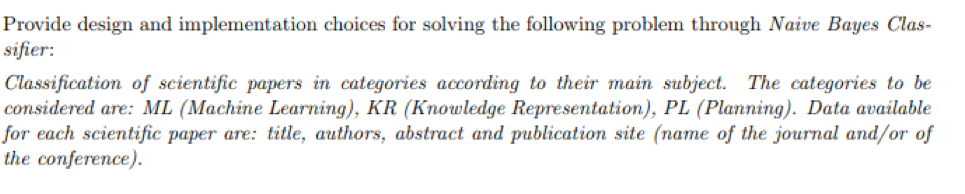
\includegraphics[scale=1]{exercises/ex1.png}
\end{figure}


In Multinomial Naïve Bayes each $p(c)$ is a multinomial distribution, so it is possible to solve the classification problem of documents using Multinomial Naïve Bayes because multinomial distribution works well for data which can easily be turned into counts, such as word counts in a text.
Given:
\begin{itemize}
\item $P(c_j)$: probability of class $c_j$
\item $P(w_i|c_j)$: probability of the word $w_i$ given the class $c_j$.
\end{itemize}
We must estimate $P(c_j)$ and $P(w_i|c_j)$ using multinomial distribution, then use them to classify a new document. Remove every word in the documents not appearing in the vocabulary V build in the previous phase and then use:
\[V_{NB}=\argmaxs{P(c_j)\prod_{i=1}^{lenght(d)}P(w_i|c_j,D)}{c_j \in C}\]

\subsection{Markov}
\begin{figure}[H]
    \centering
    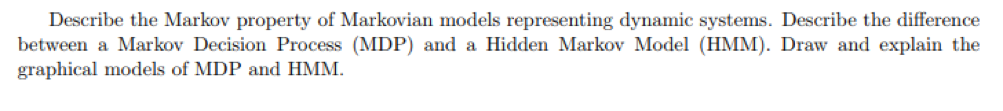
\includegraphics[scale=1]{exercises/ex2.png}
\end{figure}

\paragraph{Markov properties} once the current state is known, the evolution of the dynamic system does not depend on the history of states, actions and observations. The current state contains all the information needed to predict the future. Future states are conditionally independent of past states and past observations given the current state. The knowledge about the current state makes past, present and future observations statistically independent. Markov process has Markov properties.\\


\paragraph{MDP}
\begin{figure}[H]
    \centering
    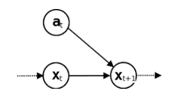
\includegraphics[scale=1]{MDP.png}
\end{figure}

An MDP is for decision making where the states are fully observable, hence there is  no need of observations. In presence of non-deterministic or stochastic actions, they can be fully observed after its execution.\\
Having 
\begin{itemize}
\item $X$ finite set of states:
\item $A$: finite set of actions
\item Deterministic $\delta: X\times A \rightarrow X$: a function which maps an action-state tuple to the next state.
\item Non-deterministic $\delta: X\times A \rightarrow 2^X$.
\item Stochastic $\delta: P(x'|x,a)$: the probability of having he state $x'$ given previous state $x$ and action $a$.
\item Deterministic $r:X\times A \rightarrow R$: a function which maps a tuple state-action to a reward.
\item Non-deterministic/Stochastic $r:X\times A \times X \rightarrow R$
\end{itemize}
An MDP is made of $MSP=\braces{X,A,\delta,r}$

\paragraph{HMM}
\begin{figure}[H]
    \centering
    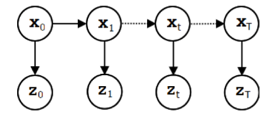
\includegraphics[scale=1]{HMM.png}
\end{figure}

In a HMM sate states $x_t$ are discrete and not observable, while the observations $z_t$ can be either discrete or continuous. Finally there is no control over the system.\\
Given:
\begin{itemize}
\item $X$: set of not observable states
\item $Z$: set of observations
\item $P(x_t|x_{t-1})$: the transition model 
\item $P(z_t|x_t)$: an observation models which maps the probability of having an observation $z_t$ to a state $x_t$.
\item $\pi_0$: an initial distribution
\item $\bm{A}=\braces{A_{ij}}=P(x_t=j|x_{t-1}=i)$ a transition matrix
\item $b_k(z_t)=P(z_t|x_t=k)$ an observation model.
\item $\pi_0=P(x_0)$: an initial probability.
\end{itemize}
We have that a HMM is made of $HMM=\braces{X,Z,\pi_0}$.

\subsection{Kernelized linear model (regression)}
\begin{figure}[H]
    \centering
    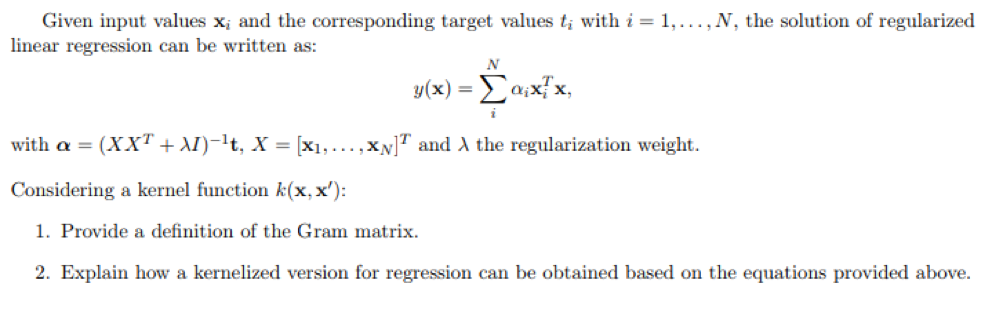
\includegraphics[scale=1]{exercises/ex3.png}
\end{figure}

\paragraph{Gram Matrix}
Given some kernel $k(x_i,x_j)$, the Gram Matrix $K=\bm{XX^T}$ is a $N\times N$ symmetric matrix of the form:
\[K_{nm}=k(x_n,x_m)\]

\paragraph{Kernalized regression}
Considering a linear kernel $k(x,x')=x^Tx'$ we can rewrite the model as:
\[y(x)=\sum_{i=1}^N\alpha_i k(x_i,x)\]
having:
\[\alpha=(K+\lambda I)^{-1}t\]

\subsection{Linear Regression}

\begin{figure}[H]
    \centering
    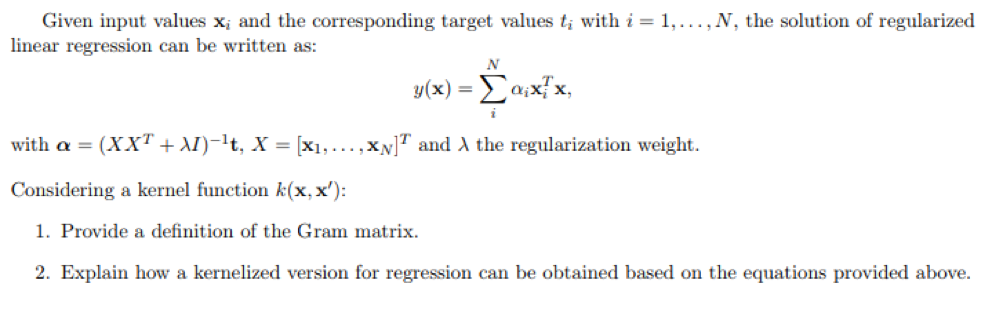
\includegraphics[scale=1]{exercises/ex3.png}
\end{figure}


\paragraph{Linear regression}
The goal of regression is to predict the value of one or more continuous target variables $Y=\mathcal{R}$ given the value of a D-dimensional vector of input variables $X \subset \mathcal{R}^D$. The simplest linear model for regression is one that involves a linear combination of the input variables:
\[y(x,w)=w_0+w_1x_1+...+w_Dx_D=\bm{w^Tx}\]
Where $x_0=1$.

\paragraph{Batch vs sequential}


We have that a target value is given by:
\[t=y(x,w) + \epsilon\]
Where $\epsilon$ is some Gaussian noise. If we assume the samples to be i.i.d. then we can use the maximum likelihood and have:
\[max[P(\braces{t_1,...,t_n}|x_1,...,x_n,w,\beta)]\]
where $\beta^{-1}$ is the variance of the noise. This approach is used with batch learning in which the entire training set is processed altogether.\\

For sequential learning \textit{stochastic gradient descent} can be used to update the model parameters in the following way:
\[w_{n+1}=w_n+\eta \nabla E_n= w_n +[t_n -w_n^T \phi(x_n)]\phi(x_n)\]
Where:
\begin{itemize}
\item $\eta$: is the learning rate 
\item $\phi(x_n)$ : is a non linear transformation of the input vector
\end{itemize}



\subsection{Linear classification}

\begin{figure}[H]
    \centering
    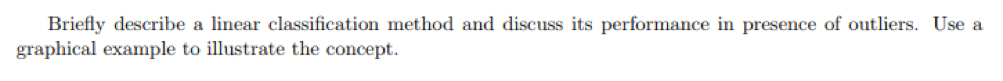
\includegraphics[scale=1]{exercises/ex5.png}
\end{figure}

The goal in classification is to take an input vector $x$ and to assign it to one of $K$  discrete classes $C_k$ where $k=1,...,K$. In the most common scenario, the classes are taken to be disjoint, so that each input is assigned to one and only one class. Data sets whose classes can be separated exactly by linear decision surfaces are said to be linearly separable. There are various ways of using target values to represent class labels.\\
For probabilistic models, the most convenient, in the case of two-class problems, is the binary representation in which there is a single target variable $t \in \braces{0,1}$ such that $t=1$ represents class $C_1$  and $t=0$  represents class $C_2$. The value of $t$ can be viewed as representing the probability of belonging to the class $C_1$.\\
For $K>2$  it is convenient to use a 1-of-K coding scheme, which is a vector $T=\braces{t_1,t_2,...,t_n}$ of length $K$ such that if the class is $C_j$, for some sample $x_i \in X,\ |X|=n$ , then the value of $t_i$ is zero everywhere except for $t_i^j$ which is one. \\
Given a dataset in the form $D=\braces{(x_n,t_n)^N_{n=1}}$ we want to find a linear discriminant $y(x)=W^Tx$, hence we minimize the sum of squares error function:
\[E(W)=\frac{1}{2}Tr\braces{(XW-T)^T(XW-T)}\]
obtaining:
\[W=(X^TX)^{-1}X^TT\]
\[y(x)=W^Tx\]
Unfortunately, least squares solutions lack robustness to outliers and are highly sensitive to them, unlike logistic regression.

\begin{figure}[H]
    \centering
    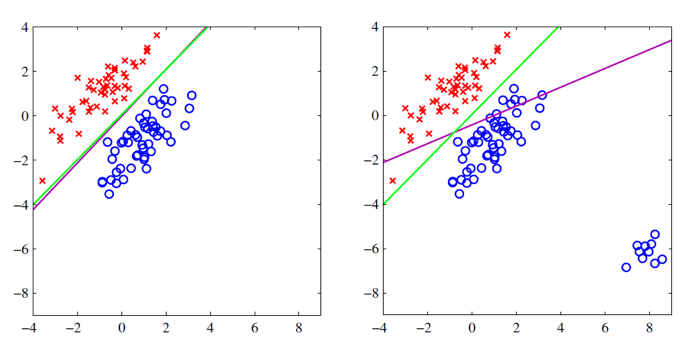
\includegraphics[scale=1]{least_square_error.png}
\end{figure}
The left plot shows data from two classes (red crosses and blue circles) with the decision boundary found by least squares (magenta) and by the logistic regression model (green). The right plot shows the corresponding results obtained when extra data points (outliers) are added at the bottom left of the diagram.

\subsection{K-NN}

\begin{figure}[H]
    \centering
    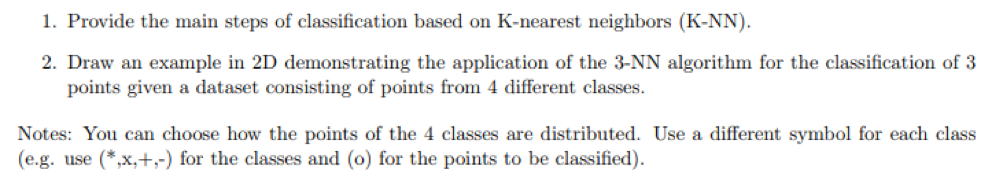
\includegraphics[scale=1]{exercises/ex6.png}
\end{figure}

\paragraph{Main steps}
Classification with K-NN, having a target function $f:X\rightarrow C$ and a dataset $D=\braces{(x_i,y_i)^N_{i=1}}$ is :
\begin{itemize}
\item Find K nearest neighbors of the new instance $x'$
\item assign $x'$ to the most common label among the majority of the neighbors.
\end{itemize}
We can estimate the likelihood of $x'$ belongign to the class $c$ as:
\[p(c| x',D,K)=\frac{1}{K}\sum_{i \in N_k(x',D)}\mathcal{I}(y_i=c)\]
with:
\begin{itemize}
\item $ N_k(x',D)$ is the set of K nearest points to $x'$
\item $\mathcal{I}(y_i=c)$ is one if the label $y_i$ is equal to $c$, zero otherwise
\end{itemize}

\paragraph{Exercise}
\begin{figure}[H]
    \centering
    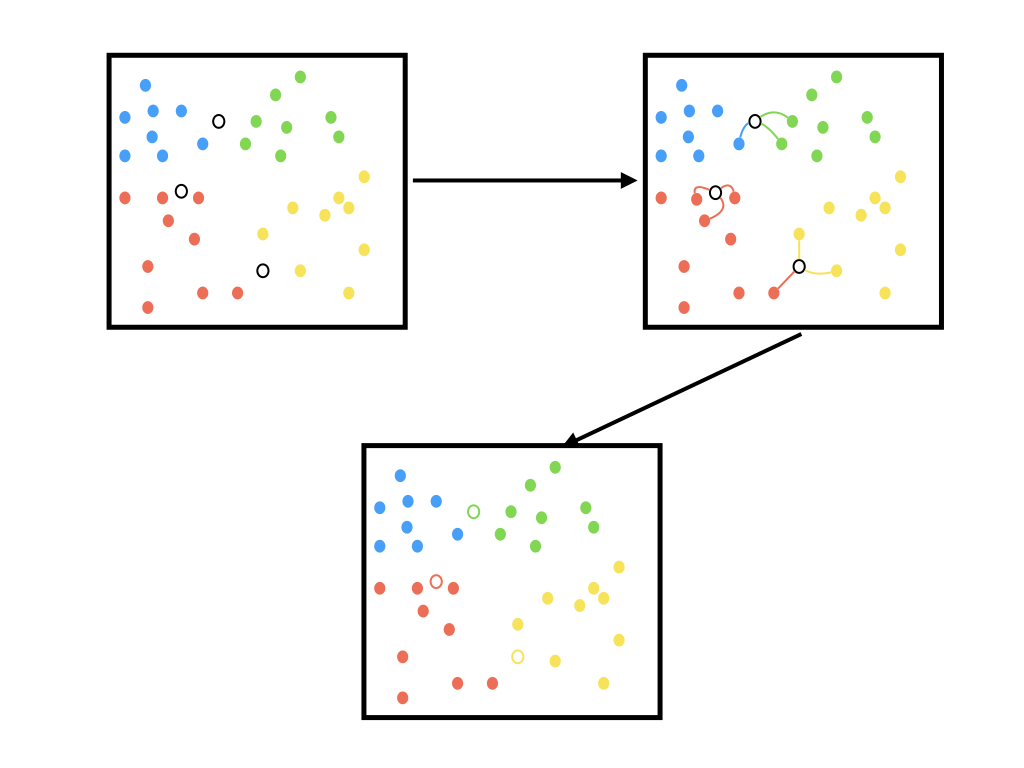
\includegraphics[scale=0.4]{knn.jpeg}
\end{figure}
\subsection{Tree classification}
\begin{figure}[H]
    \centering
    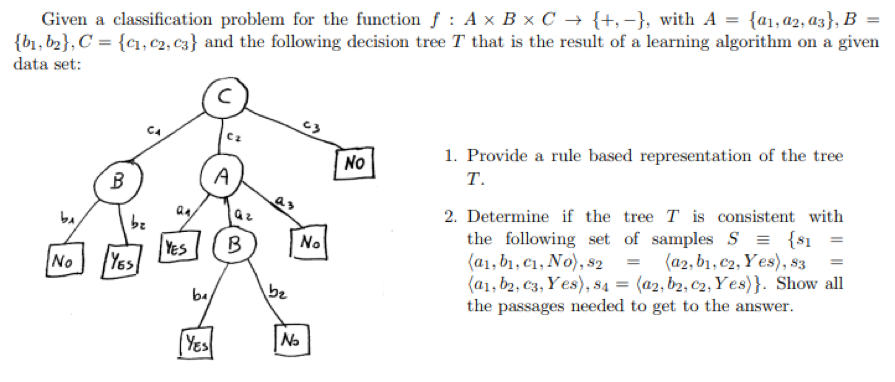
\includegraphics[scale=1]{exercises/ex7.png}
\end{figure}

\paragraph{Rules}
\begin{enumerate}

\item $c_1 \wedge b_1 \Rightarrow No $
\item $c_1 \wedge b_2 \Rightarrow Yes $
\item $c_2 \wedge a_1 \Rightarrow Yes $
\item $c_2 \wedge a_2 \wedge b_1 \Rightarrow Yes $
\item $c_2 \wedge a_2 \wedge b_2 \Rightarrow No $
\item $c_2 \wedge a_3 \Rightarrow No $
\item $c_3  \Rightarrow No $
\end{enumerate}

\paragraph{Consistency}
\begin{itemize}
\item $s_1$ is consistent because of  1 
\item $s_2$ is consistent because of  4
\item $s_3$ is not consistent because of  7 
\item $s_4$ is not consistent because of  5
\end{itemize}

\subsection{Tree overfitting}
\begin{figure}[H]
    \centering
    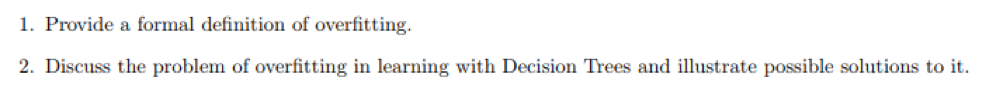
\includegraphics[scale=1]{exercises/ex8.png}
\end{figure}


\paragraph{Overfitting}
Overfitting is "the production of an analysis that corresponds too closely or exactly to a particular set of data, and may therefore fail to fit additional data or predict future observations reliably". An overfitted model is a statistical model that contains more parameters than can be justified by the data.[2] The essence of overfitting is to have unknowingly extracted some of the residual variation (i.e. the noise) as if that variation represented underlying model structure.

\paragraph{Overfitting in Tree}
Consider an hypothesis $h$ with error on the training set $error_{train}(h)$, while the error on the enitre distribution D is $error_D(h)$. The hypo $h$ overfits the training data if there is some other hypo $h'$ and the following holds:
\[error_{train}(h)<error_{train}(h')\quad and \quad error_D(h)>error_D(h')\]
stop growing when data split is not statistically significant, acquire more training data, remove irrelevant attributes, grow full tree, then post-prune. In order to select the best tree, we have to measure performance over training data, measure performance over separate validation data set, add complexity penalty to performance measure.

\subsection{Boosting}
\begin{figure}[H]
    \centering
    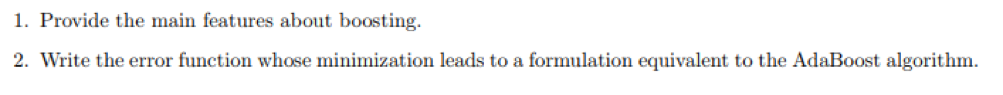
\includegraphics[scale=1]{exercises/ex9.png}
\end{figure}

\paragraph{Boosting}
In supervised learning, boosting converts weak learners to strong ones. A weak learner is defined to be a classifier that is only slightly correlated with the true classification (it can label examples better than random guessing). In contrast, a strong learner is a classifier that is arbitrarily well-correlated with the true classification.

\paragraph{AdaBoost}
No prior knowledge about base learner is required, no parameters to tune (except for M), can be combined with any method to find base learners and theoretical guarantees given enough data and base learners with moderate accuracy.\\
The error function to minimize is:
\[J_m=\sum_{n=1}^N w_n^{(m)}\mathcal{I}(y_m(x_n)\neq t_n\]
Given 
\begin{itemize}
\item $\epsilon_m = \frac{\sum_{n=1}^N w_n^{(m)}\mathcal{I}(y_m(x_n)\neq t_n}{\sum_{n=1}^N w_n^{(m)}}$
\item $\alpha=ln(\frac{1-\epsilon_m}{\epsilon_m})$
\end{itemize}
The output of the linear classifier is:
\[Y_m(x)=sign(\sum_{m=1}^M\alpha_my_m(x))\]



\end{document}
